\subsection{UC17: Gestione profilo}
\label{sec:UC17}
\begin{figure}[!ht]
    \caption{Diagramma di UC17: Gestione profilo}
    \vspace{10px}
    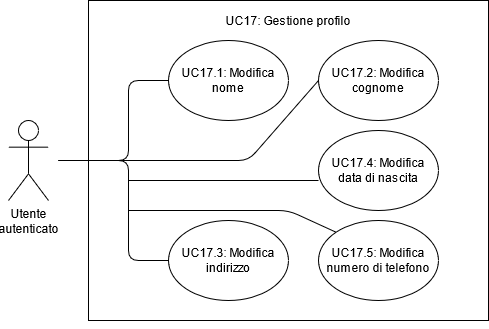
\includegraphics[scale=0.5]{../../../Images/AnalisiRequisiti/UC17}
    \centering
\end{figure}

\begin{itemize}
    \item \textbf{Descrizione:} l'utente vuole gestire il proprio profilo;
    \item \textbf{Attore Primario:} utente autenticato;
    \item \textbf{Attore Secondario:} servizio di autenticazione esterno;
    \item \textbf{Precondizione:} l'utente si trova all'interno del proprio profilo;
    \item \textbf{Postcondizione:} l'utente può modificare il proprio profilo;
    \item \textbf{Scenario Principale:}
          \begin{itemize}
              \item  l'utente decide cosa modificare tra:
                    \begin{itemize}
                        \item nome;
                        \item cognome;
                        \item username;
                        \item password;
                        \item indirizzo.
                    \end{itemize}
          \end{itemize}
\end{itemize}



\subsubsection{UC17.1 Modifica del nome}
\label{sec:UC17.1}
\begin{itemize}
    \item \textbf{Descrizione:} l'utente vuole modificare il proprio nome relativo all'account;
    \item \textbf{Attore Primario:} utente autenticato;
    \item \textbf{Attore Secondario:} servizio di autenticazione esterno;
    \item \textbf{Precondizione:} l'utente si trova all'interno del proprio profilo;
    \item \textbf{Postcondizione:} l'utente può modificare il proprio nome.
\end{itemize}

\subsubsection{UC17.2 Modifica del cognome}
\label{sec:UC17.2}
\begin{itemize}
    \item \textbf{Descrizione:} l'utente vuole modificare il proprio cognome relativo all'account;
    \item \textbf{Attore Primario:} utente autenticato;
    \item \textbf{Attore Secondario:} servizio di autenticazione esterno;
    \item \textbf{Precondizione:} l'utente si trova all'interno del proprio profilo;
    \item \textbf{Postcondizione:} l'utente può modificare il proprio cognome.
\end{itemize}

\subsubsection{UC17.3 Modifica dell'username}
\label{sec:UC17.3}
\begin{itemize}
    \item \textbf{Descrizione:} l'utente vuole modificare il proprio username;
    \item \textbf{Attore Primario:} utente autenticato;
    \item \textbf{Attore Secondario:} servizio di autenticazione esterno;
    \item \textbf{Precondizione:} l'utente si trova all'interno del proprio profilo;
    \item \textbf{Postcondizione:} l'utente può modificare il proprio username;
    \item \textbf{Estensione}: visualizzazione errore se l'username è già presente nel database \hyperref[sec:UC17.6]{UC17.6}.
\end{itemize}

\subsubsection{UC17.4 Modifica della password}
\label{sec:UC17.4}
\begin{itemize}
    \item \textbf{Descrizione:} l'utente vuole modificare la propria password;
    \item \textbf{Attore Primario:} utente autenticato;
    \item \textbf{Attore Secondario:} servizio di autenticazione esterno;
    \item \textbf{Precondizione:} l'utente si trova all'interno del proprio profilo;
    \item \textbf{Postcondizione:} l'utente può modificare la propria password.
\end{itemize}

\subsubsection{UC17.5 Modifica dell'indirizzo}
\label{sec:UC17.5}
\begin{itemize}
    \item \textbf{Descrizione:} l'utente vuole modificare il proprio indirizzo;
    \item \textbf{Attore Primario:} utente autenticato;
    \item \textbf{Attore Secondario:} servizio di autenticazione esterno;
    \item \textbf{Precondizione:} l'utente si trova all'interno del proprio profilo;
    \item \textbf{Postcondizione:} l'utente può modificare il proprio indirizzo.
\end{itemize}

\subsubsection{UC17.6: Visualizzazione username già presente}
\label{sec:UC17.6}
\begin{itemize}
    \item \textbf{Descrizione:} Visualizzazione di un errore se lo username è già in uso;
    \item \textbf{Attore Primario:} utente autenticato;
    \item \textbf{Attore Secondario:} servizio di autenticazione esterno;
    \item \textbf{Precondizione:} l'utente ha inserito uno username non disponibile perchè già usato;
    \item \textbf{Postcondizione:} l'utente visualizza un messaggio di errore.
\end{itemize}

\subsubsection{UC17.7: Password non conforme}
\label{sec:UC17.7}
\begin{itemize}
    \item \textbf{Descrizione:} Visualizzazione di un errore se la password non è conforme ai requisiti;
    \item \textbf{Attore Primario:} utente autenticato;
    \item \textbf{Attore Secondario:} Amazon Cognito;
    \item \textbf{Precondizione:} l'utente ha inserito una password non conforme ai requisiti, che sono:
          \begin{itemize}
              \item lunghezza almeno di 8 caratteri;
              \item contenga almeno una lettera maiuscola;
              \item contenga almeno una lettera minuscola;
              \item contenga almeno un numero;
              \item contenga almeno un carattere speciale.
          \end{itemize}
    \item \textbf{Postcondizione:} l'utente visualizza un messaggio di errore.
\end{itemize}